\subsection{The Sparse Readout Factorization Preserves LM-Head Behavior}

\paragraph{Replacement vs. target fidelity.}
SRP is useful as an interpretability layer only where the factorized readout
tracks the original LM head. We therefore evaluate two linked quantities:
replacement fidelity after substituting \(\widehat{\WU}\) for \(\WU\) on
held-out hidden states, and target fidelity for the pairwise logit differences
used in local feature analyses. Replacement tests whether the sparse
factorization preserves readout behavior; target fidelity tests whether the
displayed feature sums recover the selected score's size and sign.

\begin{table}[t]
\caption{\textbf{Readout replacement and target fidelity.}
cfg gives dictionary width multiplier/TopK budget. Replacement metrics use
held-out hidden states; logit-difference metrics use the main held-out target
subset. Full model names and counts are in
Appendix~\ref{app:model-suite-selection}.}
\label{tab:readout-query-fidelity-summary}
\centering
\scriptsize
\setlength{\tabcolsep}{2.0pt}
\renewcommand{\arraystretch}{1.06}
\begin{tabular}{@{}lc
S[table-format=1.3]
S[table-format=1.3]
S[table-format=1.3]
S[table-format=1.3]
S[table-format=1.3]
S[table-format=1.3]@{}}
\toprule
& & \multicolumn{3}{c}{Replacement} & \multicolumn{3}{c}{Logit differences} \\
\cmidrule(lr){3-5}\cmidrule(l){6-8}
Model & cfg & {rowEV} & {top1} & {KL} & {Sign} & {Med. \(\rho\)} & {\(\rho<0.5\)} \\
\midrule
Q-0.8B & 32/256 & 0.877 & 0.891 & 0.135 & 0.950 & 0.088 & 0.815 \\
Q-2B   & 32/256 & 0.847 & 0.887 & 0.136 & 0.958 & 0.083 & 0.829 \\
Q-9B   & 32/256 & 0.857 & 0.900 & 0.105 & 0.949 & 0.098 & 0.823 \\
\addlinespace[1pt]
G-E2B  & 32/256 & 0.834 & 0.333 & 6.37  & 0.914 & 0.269 & 0.691 \\
G-E4B  & 32/256 & 0.827 & 0.736 & 1.22  & 0.940 & 0.160 & 0.786 \\
\addlinespace[1pt]
Min-8B & 32/256 & 0.888 & 0.904 & 0.087 & \multicolumn{3}{c}{--\hspace{3pt}(replacement only)} \\
R1-Q-7B & 32/256 & 0.844 & 0.760 & 0.489 & 0.921 & 0.147 & 0.787 \\
R1-L-8B & 32/256 & 0.888 & 0.754 & 0.434 & 0.926 & 0.134 & 0.830 \\
\bottomrule
\end{tabular}
\end{table}

\paragraph{Readout and target fidelity.}
\Cref{tab:readout-query-fidelity-summary} reports row reconstruction,
replacement, and held-out logit-difference fidelity for the \(k=256\) settings
used below. We evaluate target fidelity with sign agreement, median relative error
\(\rho=|s_{\mathrm{exact}}-s_{\mathrm{recon}}|/(|s_{\mathrm{exact}}|+0.5)\),
and the fraction with \(\rho<0.5\). Qwen is strongest: replacement top-1
\(0.887\)--\(0.900\), sign agreement \(0.949\)--\(0.958\), and median
\(\rho<0.10\). Errors and sign flips concentrate near small exact margins
(\Cref{fig:readout-query-fidelity-result}); Gemma preserves signs with larger
errors. The reasoning-distilled checkpoints have lower replacement top-1/KL
but preserve contrastive signs well (sign \(0.921\)--\(0.926\), median
\(\rho<0.15\)); Appendix~\ref{app:readout-factorizer-transfer-comparisons}
expands this pattern. Target reconstruction and sign agreement calibrate the
local accounts interpreted below. RowEV remains a readout-capacity metric rather
than a sufficient condition for faithful local accounts. These metrics identify
SRP's most reliable regime: signed contrasts with nontrivial margins, with most
ambiguity concentrated in small exact margins.

\begin{figure}[t]
    \centering
    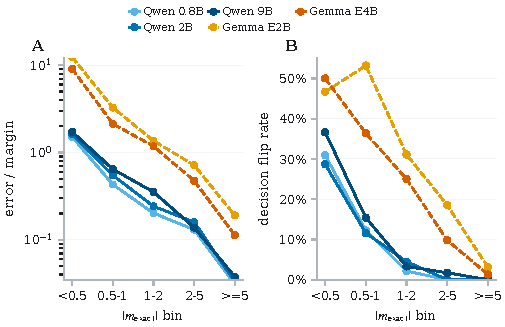
\includegraphics[width=\columnwidth]{figures/proto_token_lens/result1_query_fidelity_v2/result1_v2_five_model_margin_fidelity.pdf}
    \caption{\textbf{Held-out logit-difference fidelity.}
    (A) Median relative reconstruction error by exact-margin magnitude, with
    \(\rho=|m_{\mathrm{exact}}-m_{\mathrm{recon}}|/(|m_{\mathrm{exact}}|+0.5)\).
    (B) Decision flip rate. Flips concentrate in small-margin cases; calibration
    appears in Appendix Figure~\ref{fig:app-readout-query-margin-reconstruction}.}
    \label{fig:readout-query-fidelity-result}
\end{figure}

\subsection{Learned Token-Row Support Drives Target Reconstruction}

High-dimensional sparse bases can reconstruct some readout structure by
capacity alone. We therefore ask whether SRP's learned token-row support is
responsible for the target fidelity above.

\begin{table}[t]
\caption{\textbf{Null and reference baselines for Qwen3.5-2B.}
All methods use the full baseline/null logit-difference set: 1,348 items over
848 bootstrap base-case clusters. The last column is the fraction with preserved
sign and \(\rho<0.5\).}
\label{tab:main-baseline-null-comparison}
\centering
\scriptsize
\setlength{\tabcolsep}{3.2pt}
\renewcommand{\arraystretch}{1.06}
\begin{tabular}{@{}lccc@{}}
\toprule
Method & Med. \(\rho\) & Sign & \makecell{Sign \&\\ \(\rho<0.5\)} \\
\midrule
Sparse Readout Prism & 0.081 & 0.941 & 0.774 \\
Nearest-row ridge & 0.260 & 0.861 & 0.622 \\
PCA, 1024 dims & 0.470 & 0.829 & 0.539 \\
Shuffled sparse codes & 1.090 & 0.502 & 0.081 \\
Random support & 1.141 & 0.407 & 0.069 \\
\bottomrule
\end{tabular}
\end{table}

\paragraph{Support controls.}
On the full Qwen3.5-2B logit-difference set, SRP has the lowest median error and
largest sign-preserved low-error subset
(\Cref{tab:main-baseline-null-comparison}).
Nearest-row ridge \citep{hoerl1970ridge} and PCA \citep{jolliffe2002principal}
references retain some sign structure, while shuffled codes and random supports
approach chance, indicating dependence on learned token-to-feature support. The
full error tail appears in
Appendix~\ref{app:robustness-key-quantitative}.
Thus the sparse code support learned from vocabulary rows, not merely the
availability of a large basis, drives the reconstruction used by the local
accounts.

\subsection{Scalar Readout Targets Extend Beyond Token Pairs}

The scalar-target interface is not tied to hand-picked token pairs. The same
accounting identity applies to any linear combination of vocabulary rows, so we
instantiate task-shaped readout targets for QA
\citep{rajpurkar2018squad2,yang2018hotpotqa}, abstention, ContractNLI labels
through LegalBench \citep{koreeda2021contractnli,guha2023legalbench}, and
SecurityEval safe/unsafe actions \citep{siddiq2022securityeval}. These targets
test whether SRP reconstructs decision-shaped readout contrasts while keeping
the evaluation at the readout level.

\Cref{tab:benchmark-derived-task-targets} shows sign reconstruction on
Qwen3.5-0.8B and Qwen3.5-2B. Qwen3.5-2B is strongest on answerable QA,
multi-hop distractors, and legal labels; SecurityEval is harder because its
safe/unsafe-action contrast is diffuse. These rows isolate readout-target
fidelity and should not be read as benchmark task accuracy.
\Cref{fig:benchmark-task-group-examples} shows representative low-error QA
accounts.

\begin{table}[t]
\caption{\textbf{Benchmark-format readout-target fidelity.}
Rows evaluate benchmark-format scalar targets: answer versus distractor,
abstention versus entity, label contrast, or safe versus unsafe action. The last
column reports sign agreement with \(\rho<0.5\), where
\(\rho=|s_{\mathrm{exact}}-s_{\mathrm{recon}}|/(|s_{\mathrm{exact}}|+0.5)\).
All rows aggregate 300 targets; family rows break down Qwen3.5-2B.}
\label{tab:benchmark-derived-task-targets}
\centering
\scriptsize
\setlength{\tabcolsep}{3.0pt}
\renewcommand{\arraystretch}{1.05}
\begin{tabular}{@{}llrrrr@{}}
\toprule
Model & Target source & \(n\) & Med. \(\rho\) & Sign & \makecell{Sign \&\\ \(\rho<.5\)} \\
\midrule
Q-0.8B & all task targets & 300 & 0.180 & 0.983 & 0.933 \\
Q-2B & all task targets & 300 & 0.129 & 0.943 & 0.840 \\
\addlinespace[1pt]
Q-2B & SQuAD2 answerable & 50 & 0.150 & 1.000 & 0.900 \\
Q-2B & HotpotQA distractor & 75 & 0.125 & 0.933 & 0.907 \\
Q-2B & LegalBench ContractNLI & 50 & 0.053 & 1.000 & 1.000 \\
Q-2B & SQuAD2 unanswerable & 75 & 0.157 & 0.920 & 0.787 \\
Q-2B & SecurityEval & 50 & 0.393 & 0.880 & 0.600 \\
\bottomrule
\end{tabular}
\end{table}

\begin{figure}[t]
    \centering
    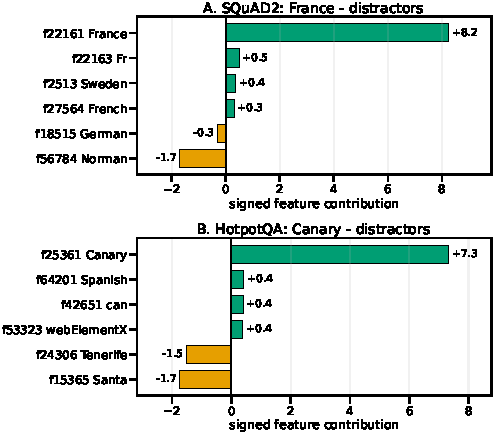
\includegraphics[width=\columnwidth]{figures/proto_token_lens/benchmark_task_group_targets/benchmark_task_group_examples.pdf}
\caption{\textbf{Benchmark-format local score accounts.}
    Positive bars support the gold/intended side; negative bars support the
    distractor side. Both Qwen3.5-2B panels use the selected \(32\times\),
    \(k=256\) readout SAE and have correct sign with low relative error. Feature
    labels summarize the highest-activating unembedding rows.}
    \label{fig:benchmark-task-group-examples}
\end{figure}
